\subsection{Activity recognition on unseen participants}
The UCI Human Activity Recognition data contain 561 summary features of motion-sensor windows during six activities~\citep{reyesortiz2013har}. Adjacent windows overlap within participants. We used the official split of 7,352 windows from 21 training participants and 2,947 windows from nine different test participants. Each of the nine contributed examples of all six activities. We averaged recalls across activities within each participant and then equally across the nine participants. Three prespecified algorithm seeds resample features or witnesses on the same training set. They do not increase the number of test participants. The experiment used one ranking per seed at five fixed fractions, corresponding to 6, 29, 57, 141 and 281 columns.

\begin{figure}[tbp]
\centering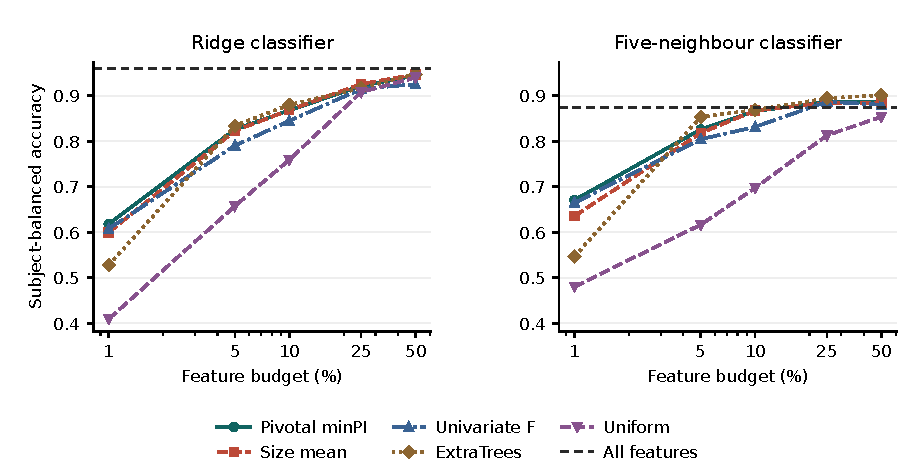
\includegraphics[width=\linewidth]{figures/subject-transfer}
\caption{UCI HAR accuracy balanced over six activities within each of nine unseen participants, then averaged equally across participants and over three algorithm seeds. The full-width reference uses 561 features for both learners.}
\label{fig:har}
\end{figure}
At six columns, voting attained 0.618 balanced accuracy with ridge and 0.671 with five-neighbour classification. Both were the highest values among the equal-budget rankings, tied by the largest layer alone. At 57 columns the voting scores were 0.868 and 0.866, compared with 0.845 and 0.832 for $F$ selection, and 0.880 and 0.869 for tree-impurity ranking (Fig.~\ref{fig:har}). Full-width ridge reached 0.959, while the full-width neighbour classifier reached 0.875. Thus the cost in predictive quality at a fixed width depends on the learner even on the same nine people. At 57 columns, voting exceeded $F$ for eight of nine subjects with each learner. For the remaining subject its balanced accuracy fell by 0.215 with ridge and by 0.070 with five neighbours. The size mean reached 0.869 and 0.867, respectively. For every budget and seed, the largest layer alone produced exactly the voting rule's support and predictions.
